\subsection{Produktintegrationsmethode}

\begin{align}
    \frac{\mathrm{d}}{\mathrm{d}x} (u(x) \cdot v(x)) &= u(x) \cdot v'(x) + u'(x) \cdot v(x) \\
    \int \frac{\mathrm{d}}{\mathrm{d}x} (u(x) \cdot v(x)) \;\mathrm{d}x &= u(x) \cdot v(x) + C = \int u(x) \cdot v'(x) \;\mathrm{d}x + \int u'(x) \cdot v(x) \;\mathrm{d}x
\end{align}

\begin{gesetz}
    \[
        \int u(x) \cdot v'(x) \;\mathrm{d}x = u(x) \cdot v(x) - \int u'(x) \cdot v(x) \;\mathrm{d}x  
    \]
\end{gesetz}

\begin{hilfe}
    \textbf{Beispielrechnung}
    \begin{figure}[H]
        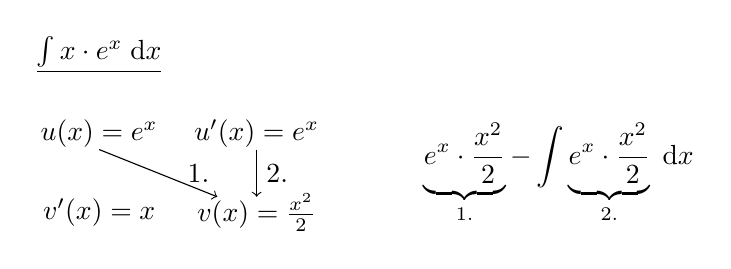
\begin{tikzpicture}
            \node at (0, 2) {\( \underline{\int x \cdot e^x \;\mathrm{d}x} \)};
            
            \node at (0, 1) {\( u(x) = e^x \)};
            \node at (2, 1) {\( u'(x) = e^x \)};
            \node at (0, 0) {\( v'(x) = x \)};
            \node at (2, 0) {\( v(x) = \frac{x^2}{2} \)};
            
            \draw[->] (0, 0.8) -- (1.5, 0.2);
            \node[right] at (1, 0.5) { 1. };
            \draw[->] (2, 0.8) -- (2, 0.2);
            \node[right] at (2, 0.5) { 2. };
            
            % \node[right] at (4, 1) {\( \displaystyle u(x) \cdot v(x) - \int u'(x) \cdot v(x) \;\mathrm{d}x \)};
            \node[right] at (4, 0.5) {\( \displaystyle \underbrace{e^x \cdot \frac{x^2}{2}}_{\text{1.}} - \int \underbrace{e^x \cdot \frac{x^2}{2}}_{\text{2.}} \;\mathrm{d}x \)};
        \end{tikzpicture}
    \end{figure}
\end{hilfe}

\paragraph{Beispiel}

\begin{align*}
    &\int x \cdot e^x \;\mathrm{d}x && \\
    \\
    &\begin{array}{ll}
        u(x) = e^x & u'(x) = e^x \\
        v'(x) = x & v(x) = \frac{x^2}{2} 
    \end{array} \\
    \\
    &\Rightarrow{} e^x \cdot \frac{x^2}{2}- \int{}e^x \cdot \frac{x^2}{x} \;\mathrm{d}x \\
    \\
    &\begin{array}{ll}
        u(x) = x & u'(x) = 1 \\
        v'(x) = e^x & v(x) = e^x \\
    \end{array} \\
    \\
    &\Rightarrow{} x \cdot e^x- \int{}e^x \;\mathrm{d}x
    %       \\
    %     &= x \cdot e^x - e^x + C \\
    %     &= e^x (x - 1) + C
\end{align*}
